%----------------------------------------------------------------------
%  Chapter 85 — Comprehensive Cyclic Multiscale Validation
%----------------------------------------------------------------------
\chapter{Comprehensive Cyclic Multiscale Validation}
\label{ch:cyclic-multiscale-validation}

This chapter presents a systematic multi-level validation of the cyclic
response of a reinforced-concrete column, from uniaxial material
behaviour up to the FE$^2$ multiscale formulation.
Every level is compared with its neighbour to build a chain of trust
that links the lowest-scale model (material point) to the
highest-scale structural simulation.

%======================================================================
\section{Problem Definition}
\label{sec:v2-problem}
%======================================================================

\subsection{Column Geometry and Reinforcement}
\label{ssec:v2-geometry}

A rectangular cantilever column is studied with the following properties:

\begin{table}[htbp]
\centering
\caption{Column properties for the V2 validation campaign.}
\label{tab:v2-column}
\begin{tabular}{@{}lrl@{}}
\toprule
\textbf{Parameter}             & \textbf{Value} & \textbf{Unit} \\
\midrule
Height $H$                     & 4.0    & m     \\
Cross-section width $B_x$      & 0.50   & m     \\
Cross-section depth $B_y$      & 0.30   & m     \\
Cover $c$                      & 0.04   & m     \\
Concrete strength $f'_c$       & 28     & MPa   \\
Steel yield stress $f_y$       & 420    & MPa   \\
Steel elastic modulus $E_s$    & 200\,000 & MPa \\
Longitudinal bars              & 12\#6  & —     \\
\bottomrule
\end{tabular}
\end{table}

The cross-section layout is shown in Figure~\ref{fig:v2-cross-section}.
The twelve reinforcing bars are arranged as four corner bars, four
intermediate bars along the top and bottom faces, two along each
short face, and two along each long face between corners.

\begin{figure}[htb]
\centering
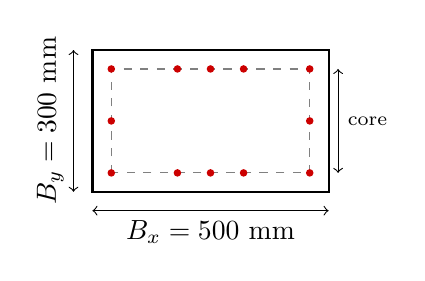
\begin{tikzpicture}[scale=6.0]
  % Concrete outline
  \draw[thick] (0,0) rectangle (0.50,0.30);
  % Cover line
  \draw[dashed, gray] (0.04,0.04) rectangle (0.46,0.26);
  % Reinforcing bars (12 total, filled circles)
  \foreach \x/\y in {%
    0.04/0.04, 0.04/0.26,           % left corners
    0.46/0.04, 0.46/0.26,           % right corners
    0.18/0.04, 0.32/0.04,           % bottom face
    0.18/0.26, 0.32/0.26,           % top face
    0.04/0.15,                       % left face mid
    0.46/0.15,                       % right face mid
    0.25/0.04, 0.25/0.26%           % extra face bars
  }{
    \fill[red!80!black] (\x,\y) circle (0.008);
  }
  % Dimensions
  \draw[<->] (0,-0.04) -- (0.50,-0.04)
    node[midway, below] {$B_x = 500$~mm};
  \draw[<->] (-0.04,0) -- (-0.04,0.30)
    node[midway, left, rotate=90, anchor=south] {$B_y = 300$~mm};
  \draw[<->] (0.50+0.02,0.04) -- (0.50+0.02,0.26)
    node[midway, right, font=\scriptsize] {core};
\end{tikzpicture}
\caption{Cross-section layout with 12 longitudinal bars.
  Dashed line: confined core boundary (cover~$=40$~mm).}
\label{fig:v2-cross-section}
\end{figure}

\subsection{Loading Protocols}
\label{ssec:v2-protocols}

Two quasi-static cyclic displacement protocols are applied at the
column tip.  Each level is a full symmetric triangle
$0 \to +A \to -A \to 0$ and the amplitude increases monotonically.

\begin{table}[htbp]
\centering
\caption{Cyclic loading protocol amplitudes.}
\label{tab:v2-protocols}
\begin{tabular}{@{}lll@{}}
\toprule
\textbf{Protocol} & \textbf{Levels (mm)} & \textbf{Peak drift (\%)} \\
\midrule
Extended\,50  & 0.5, 1, 2, 5, 10, 20, 30, 50       & 1.25 \\
Extended\,100 & 2.5, 5, 10, 20, 30, 50, 60, 80, 100 & 2.5  \\
\bottomrule
\end{tabular}
\end{table}

Each amplitude level~$A_k$ is subdivided into $n_\text{sub}$
sub-steps with a three-segment ramp:
\begin{equation}
  u(p) = A_k \times
  \begin{cases}
    4p,       & 0 \le p < \tfrac14, \\
    2 - 4p,   & \tfrac14 \le p < \tfrac34, \\
    4p - 4,   & \tfrac34 \le p \le 1,
  \end{cases}
  \label{eq:cyclic-ramp}
\end{equation}
where $p \in [0,1]$ is the normalised pseudo-time within each level.


%======================================================================
\section{Material Characterisation}
\label{sec:v2-materials}
%======================================================================

\subsection{Concrete: Kent--Park Model}
\label{ssec:v2-kent-park}

The uniaxial Kent--Park model captures the confined and unconfined
compressive envelope, linear tension cut-off, and cyclic stiffness
degradation.  The stress--strain envelope in compression reads:
\begin{equation}
  \sigma_c(\varepsilon) =
  \begin{cases}
    f'_c \left[
      \dfrac{2\varepsilon}{\varepsilon_0}
      - \left(\dfrac{\varepsilon}{\varepsilon_0}\right)^{\!2}
    \right], & |\varepsilon| \le \varepsilon_0, \\[6pt]
    f'_c \bigl[1 - Z(\varepsilon - \varepsilon_0)\bigr],
      & |\varepsilon| > \varepsilon_0,
  \end{cases}
  \label{eq:kent-park}
\end{equation}
with $\varepsilon_0 = 0.002$ for unconfined concrete and
$Z = 0.5 / (\varepsilon_{50u} + \varepsilon_{50h} - \varepsilon_0)$.

\begin{figure}[htbp]
  \centering
  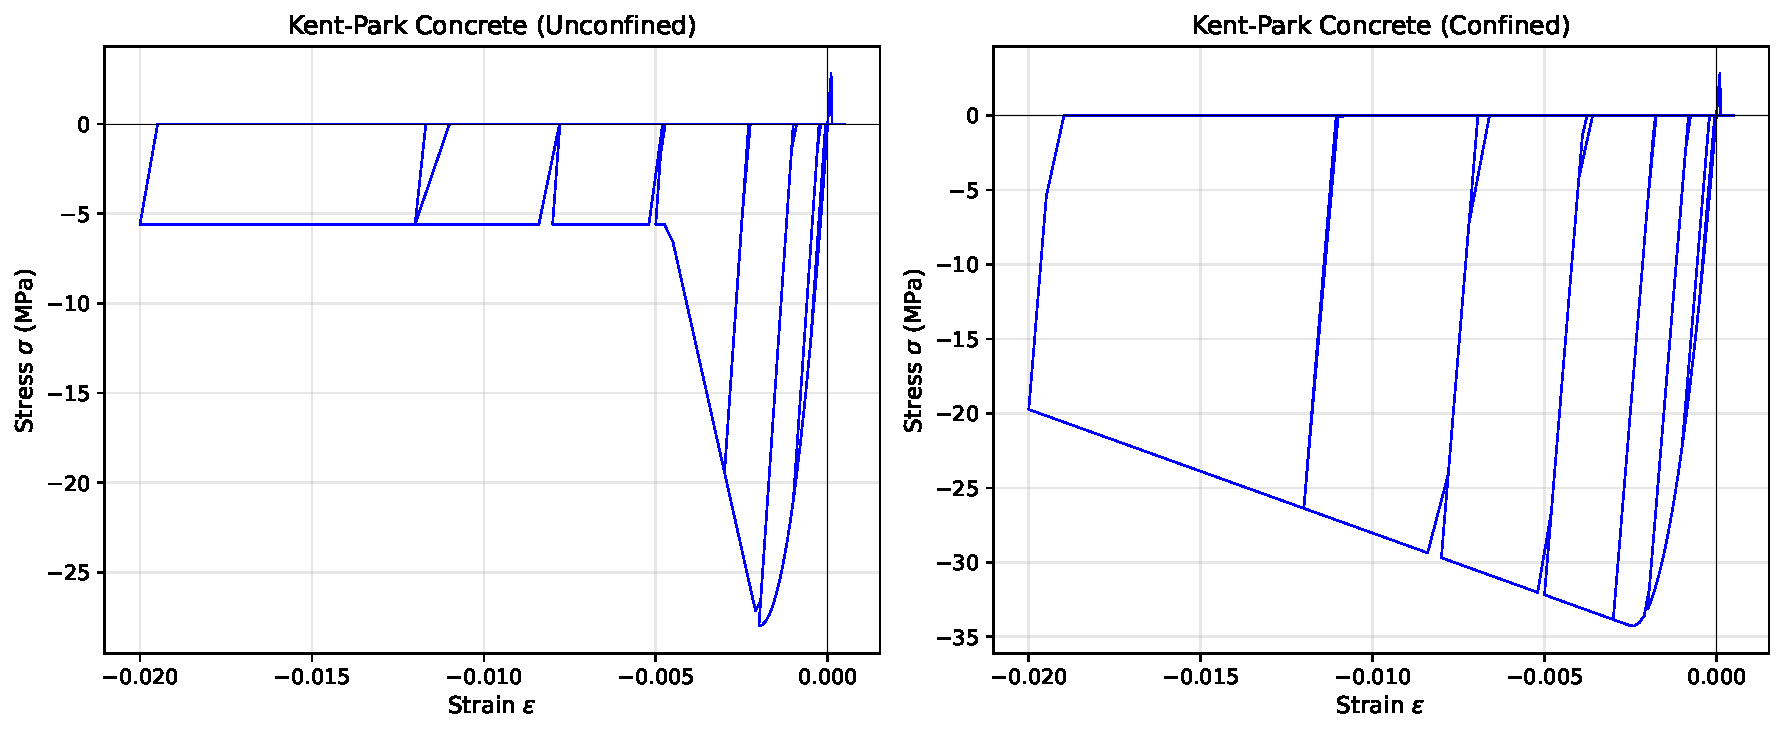
\includegraphics[width=0.92\textwidth]{figures/cyclic_validation_v2/material_concrete_hysteresis.pdf}
  \caption{%
    Kent--Park concrete cyclic stress--strain response.
    Left: unconfined ($K=1$).  Right: confined ($K>1$).%
  }
  \label{fig:v2-concrete-hysteresis}
\end{figure}

\subsection{Steel: Menegotto--Pinto Model}
\label{ssec:v2-menegotto-pinto}

The Menegotto--Pinto model with isotropic hardening captures the
Bauschinger effect observed in cyclic tests of reinforcing steel:
\begin{equation}
  \sigma^* = b\,\varepsilon^*
    + \frac{(1-b)\,\varepsilon^*}{
      \bigl(1 + |\varepsilon^*|^R\bigr)^{1/R}
    },
  \label{eq:menegotto-pinto}
\end{equation}
where $\sigma^* = (\sigma - \sigma_r)/(\sigma_0 - \sigma_r)$,
$\varepsilon^* = (\varepsilon - \varepsilon_r)/(\varepsilon_0 - \varepsilon_r)$,
$b$~is the hardening ratio, and
$R = R_0 - a_1\xi/(a_2 + \xi)$~controls the curvature of the
transition curve.

\begin{figure}[htbp]
  \centering
  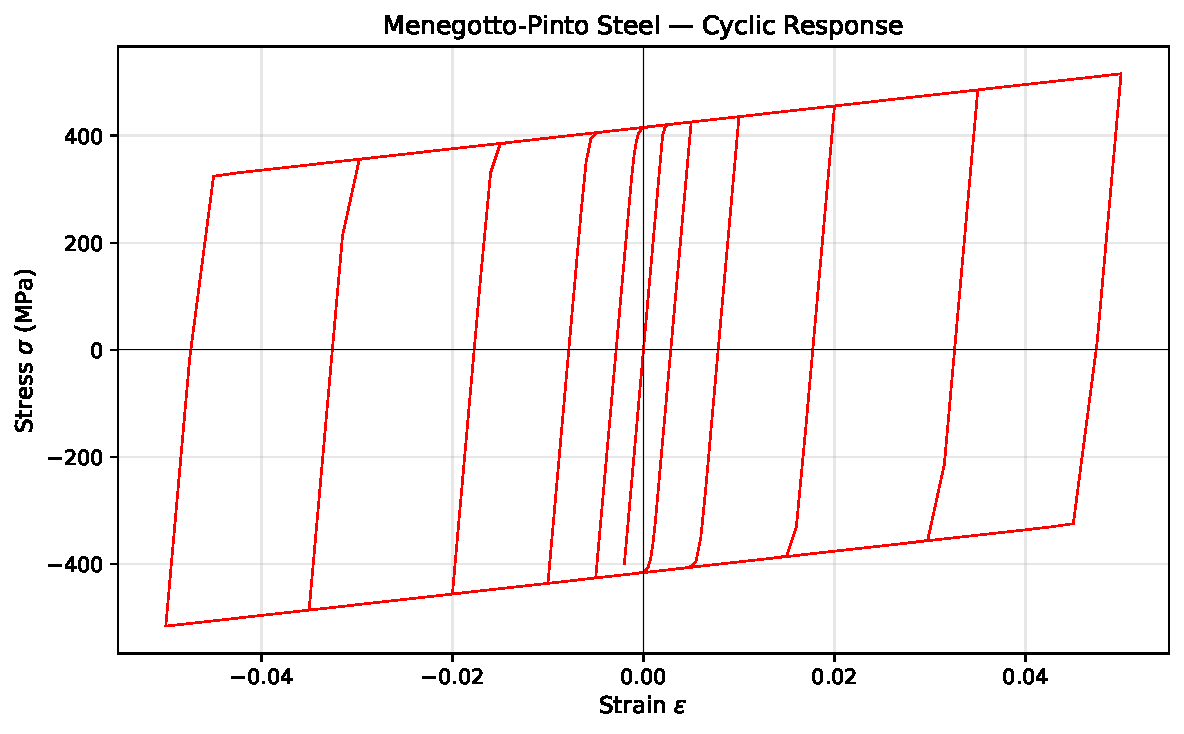
\includegraphics[width=0.72\textwidth]{figures/cyclic_validation_v2/material_steel_hysteresis.pdf}
  \caption{%
    Menegotto--Pinto steel cyclic stress--strain response
    with Bauschinger effect.%
  }
  \label{fig:v2-steel-hysteresis}
\end{figure}

\subsection{Energy Dissipation Comparison}
\label{ssec:v2-energy}

Figure~\ref{fig:v2-energy} plots cumulative energy density
$W = \int_0^t \sigma\,\dd\varepsilon$ accumulated through the cyclic
protocol for all three material models.

\begin{figure}[htbp]
  \centering
  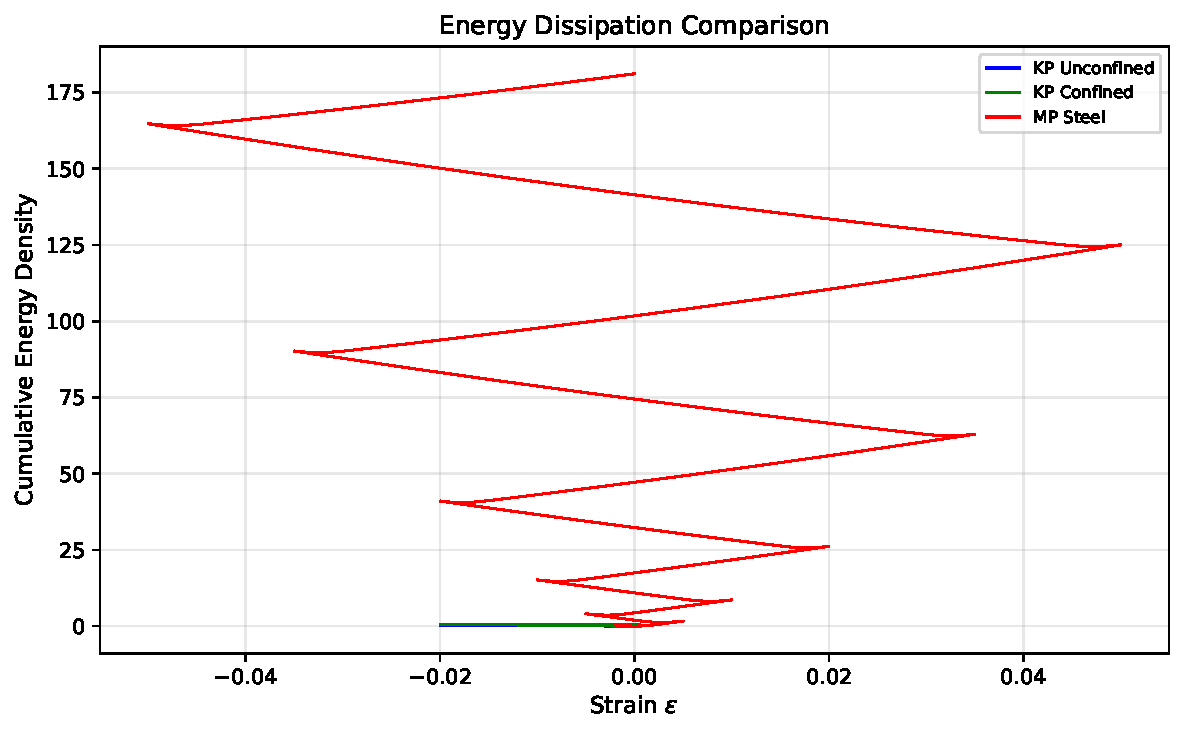
\includegraphics[width=0.72\textwidth]{figures/cyclic_validation_v2/material_energy_comparison.pdf}
  \caption{%
    Cumulative dissipated energy density for the three material models.%
  }
  \label{fig:v2-energy}
\end{figure}


%======================================================================
\section{Fiber Section Analysis}
\label{sec:v2-section}
%======================================================================

The moment--curvature ($M$--$\kappa$) response of the V2 column
cross-section is obtained by driving the \texttt{FiberSection3D}
with prescribed generalised strains.
The section integration uses a patch discretization of the cross-section
(10$\times$2 cover patches + 8$\times$6 confined-core grid) with
12 discrete rebar fibers at the bar positions shown in
Figure~\ref{fig:v2-cross-section}.

\subsection{Monotonic Push}
\label{ssec:v2-mk-mono}

Figure~\ref{fig:v2-mk-mono} shows the monotonic moment--curvature
response for both strong-axis ($M_z$, bending about $z$) and
weak-axis ($M_y$) loading.
The yield curvature $\kappa_y$ is identified as the point where the
tangent stiffness drops below 90\% of the initial elastic value.

\begin{figure}[htbp]
  \centering
  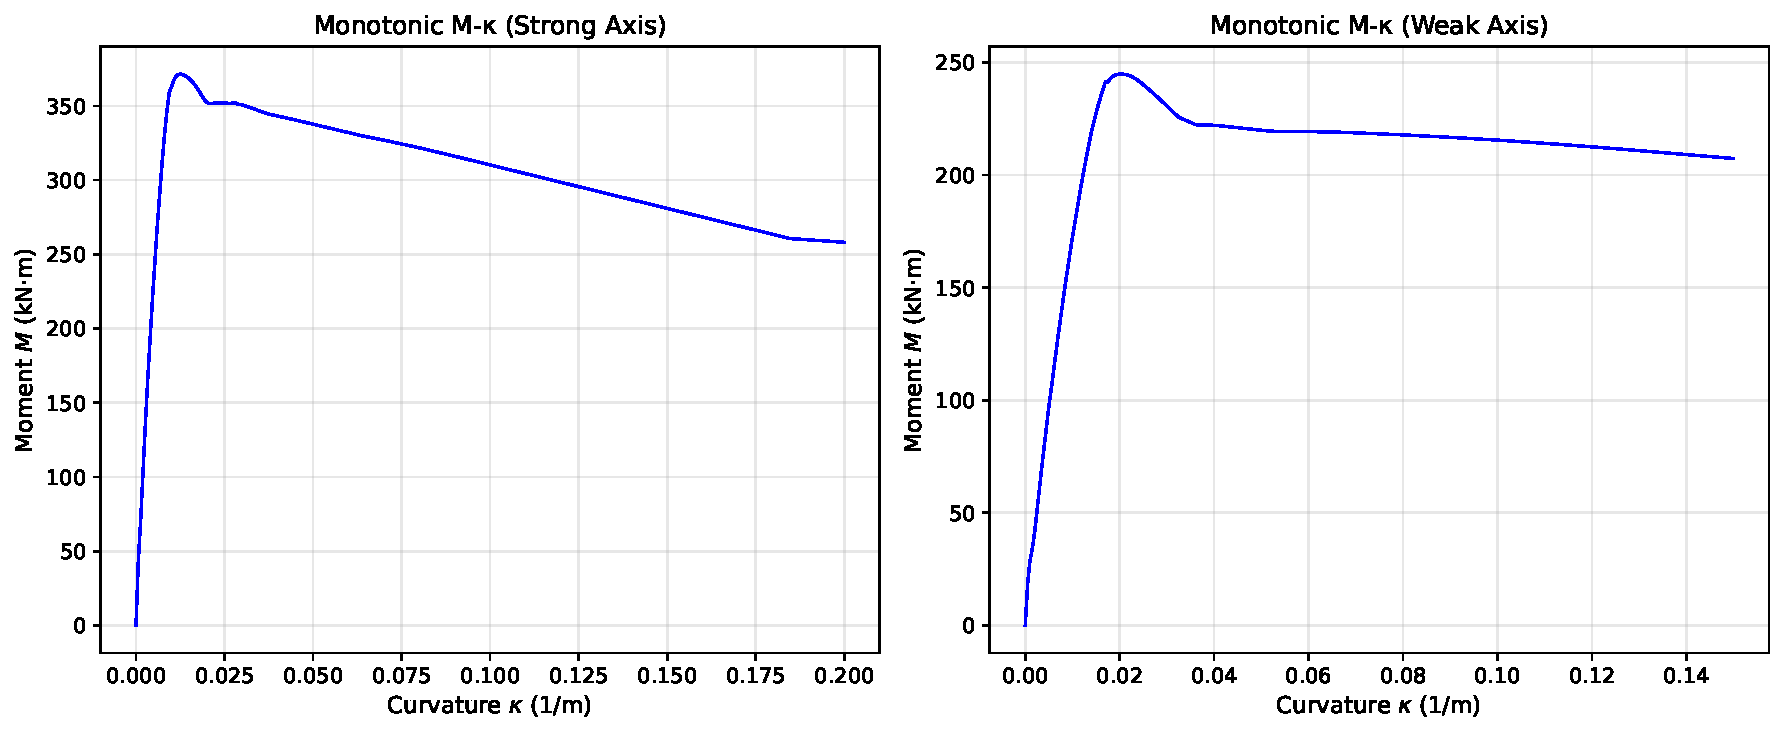
\includegraphics[width=0.92\textwidth]{figures/cyclic_validation_v2/section_mk_monotonic.pdf}
  \caption{%
    Monotonic moment--curvature response.
    Left: strong axis.  Right: weak axis.%
  }
  \label{fig:v2-mk-mono}
\end{figure}

\subsection{Cyclic Loading}
\label{ssec:v2-mk-cyclic}

The same section is subjected to the Extended\,50 cyclic curvature
protocol rescaled to curvature amplitudes up to $\pm 0.05$~m$^{-1}$.
Figures~\ref{fig:v2-mk-cyclic} show the resulting hysteresis loops.

\begin{figure}[htbp]
  \centering
  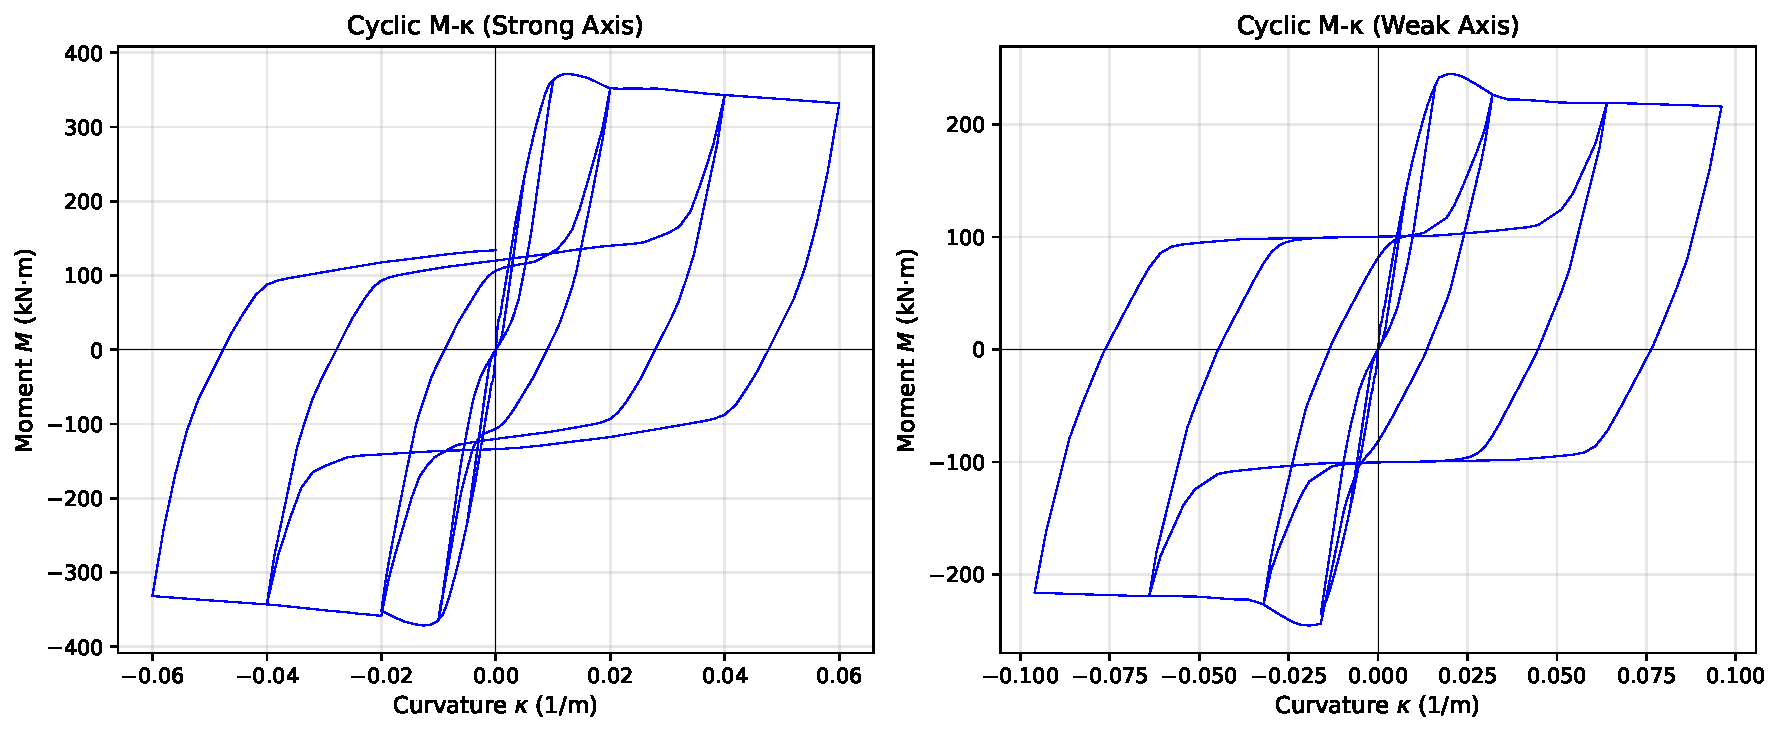
\includegraphics[width=0.92\textwidth]{figures/cyclic_validation_v2/section_mk_cyclic.pdf}
  \caption{%
    Cyclic moment--curvature response.
    Left: strong axis.  Right: weak axis.%
  }
  \label{fig:v2-mk-cyclic}
\end{figure}


%======================================================================
\section{Beam Element Convergence}
\label{sec:v2-beam}
%======================================================================

Nine cantilever models are constructed using Timoshenko beam elements
with $N=2,3,\ldots,10$ nodes per element (MITC locking-free
formulation with $(N-1)$-point Gauss--Lobatto integration).
All share the same fiber cross-section and loading protocol.

\subsection{Force--Displacement Overlay}
\label{ssec:v2-beam-overlay}

Figure~\ref{fig:v2-beam-overlay} overlays the base-shear versus
tip-drift hysteresis for every $N$.  The $N=2$ and $N=3$ models
complete all 180~steps, while $N \ge 4$ models abort progressively
earlier due to strain localization at cracking onset.

\begin{figure}[htbp]
  \centering
  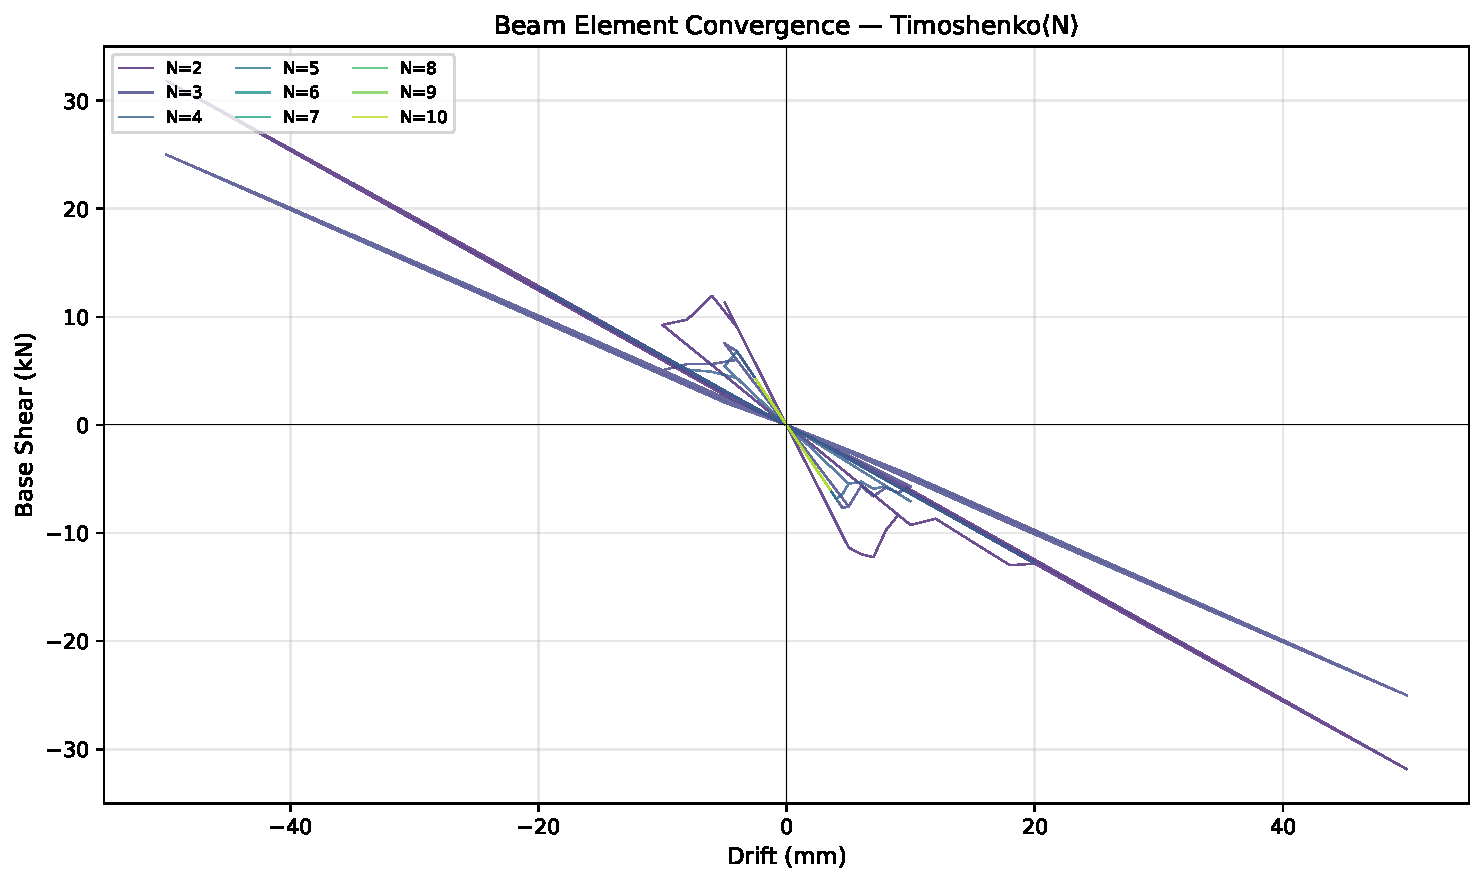
\includegraphics[width=0.92\textwidth]{figures/cyclic_validation_v2/beam_convergence_overlay.pdf}
  \caption{%
    Beam element convergence: base shear versus tip drift
    for Timoshenko$\langle N\rangle$, $N=2\ldots10$.%
  }
  \label{fig:v2-beam-overlay}
\end{figure}

\subsection{Convergence Curve}
\label{ssec:v2-beam-convergence}

Figure~\ref{fig:v2-beam-conv} plots the peak base shear as a function
of the number of element nodes $N$.  Due to the early aborts for
$N \ge 4$, the peak shear decreases with increasing $N$, reflecting
the reduced drift range rather than converged capacity.  The result
reveals the tension between interpolation richness and strain
localization for softening materials.

\begin{figure}[htbp]
  \centering
  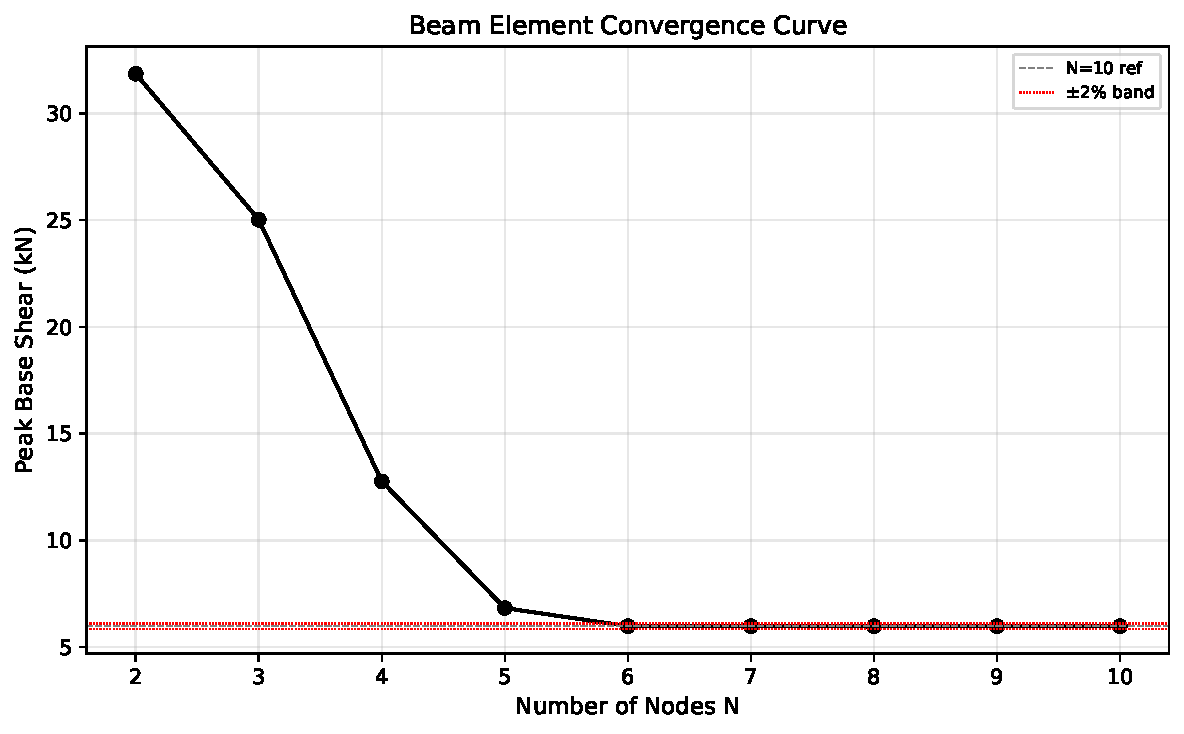
\includegraphics[width=0.72\textwidth]{figures/cyclic_validation_v2/beam_convergence_curve.pdf}
  \caption{%
    Peak base shear convergence curve.
    Dashed line: $N=10$ reference.
    Red band: $\pm 2\%$ tolerance.%
  }
  \label{fig:v2-beam-conv}
\end{figure}


%======================================================================
\section{Continuum Element Mesh Study}
\label{sec:v2-continuum}
%======================================================================

The same column is modelled with three hexahedral element types
(Hex8, Hex20, Hex27) each at three mesh densities ($n_x \times n_y
\times n_z$ divisions).  The Ko--Bathe three-dimensional concrete model
is used with embedded rebar via penalty coupling
($\alpha = 10\,E_c$).

\begin{table}[htbp]
\centering
\caption{Continuum mesh configurations.}
\label{tab:v2-mesh}
\begin{tabular}{@{}llrrrl@{}}
\toprule
\textbf{Type} & \textbf{Density} & $n_x$ & $n_y$ & $n_z$ & \textbf{DOFs (approx)} \\
\midrule
Hex8   & coarse  & 4 & 3 & 8   & $\sim$500  \\
Hex8   & medium  & 6 & 4 & 16  & $\sim$1\,700 \\
Hex8   & fine    & 8 & 6 & 24  & $\sim$4\,200 \\
\midrule
Hex20  & coarse  & 2 & 2 & 4   & $\sim$300  \\
Hex20  & medium  & 4 & 3 & 8   & $\sim$1\,800 \\
Hex20  & fine    & 6 & 4 & 12  & $\sim$6\,000 \\
\midrule
Hex27  & coarse  & 2 & 2 & 4   & $\sim$500  \\
Hex27  & medium  & 3 & 2 & 6   & $\sim$1\,400 \\
Hex27  & fine    & 4 & 3 & 8   & $\sim$3\,600 \\
\bottomrule
\end{tabular}
\end{table}

\subsection{Per-Element-Type Convergence}
\label{ssec:v2-hex-conv}

Figures~\ref{fig:v2-hex8}--\ref{fig:v2-hex27} show the base-shear
versus tip-drift hysteresis for each element type at three mesh densities.

\begin{figure}[htbp]
  \centering
  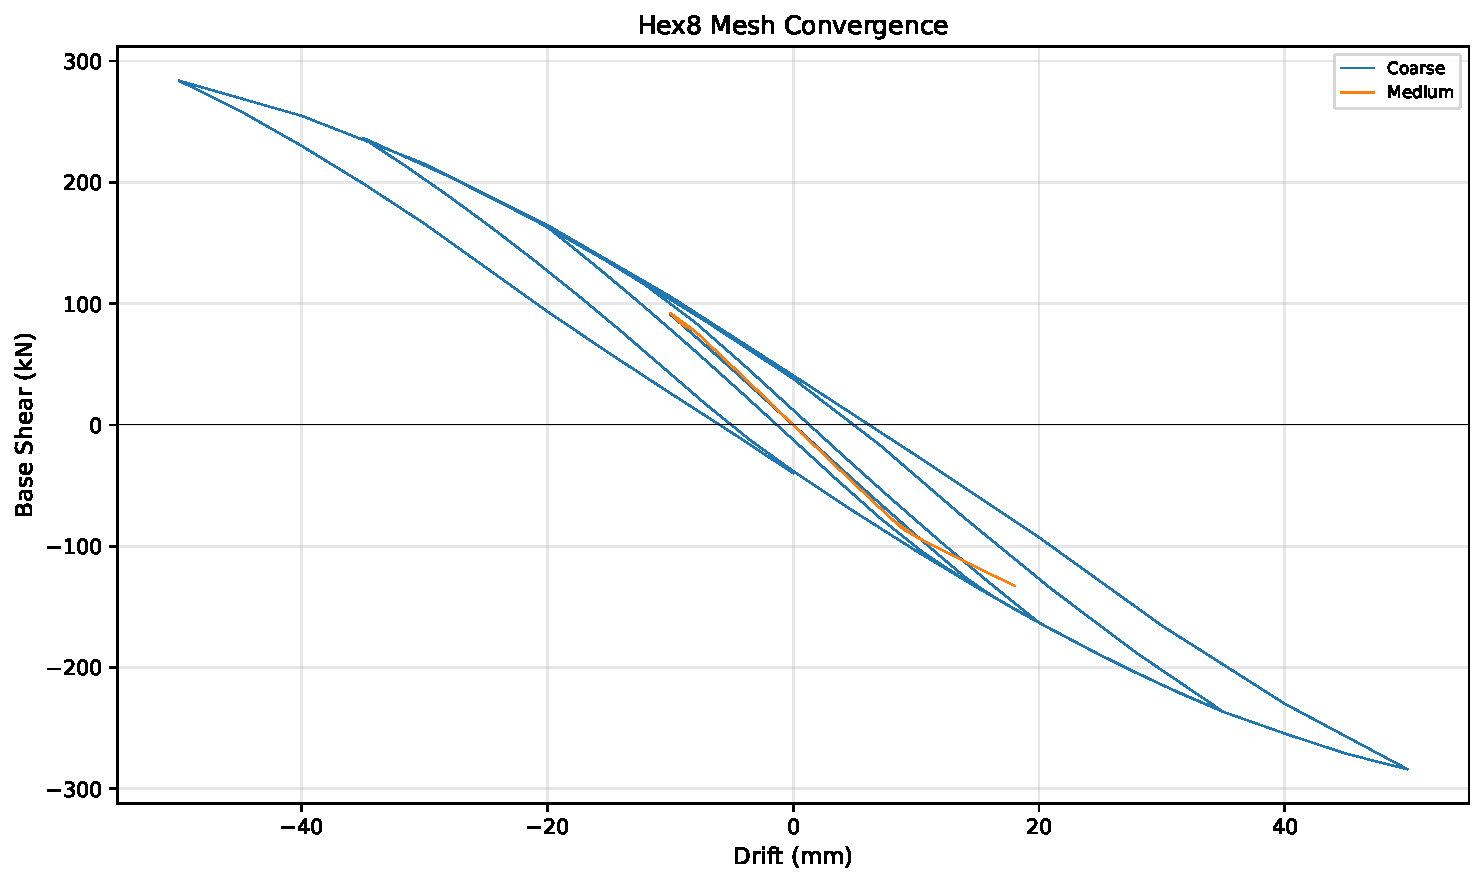
\includegraphics[width=0.92\textwidth]{figures/cyclic_validation_v2/hex8_mesh_convergence.pdf}
  \caption{Hex8 mesh convergence (coarse / medium / fine).}
  \label{fig:v2-hex8}
\end{figure}

\begin{figure}[htbp]
  \centering
  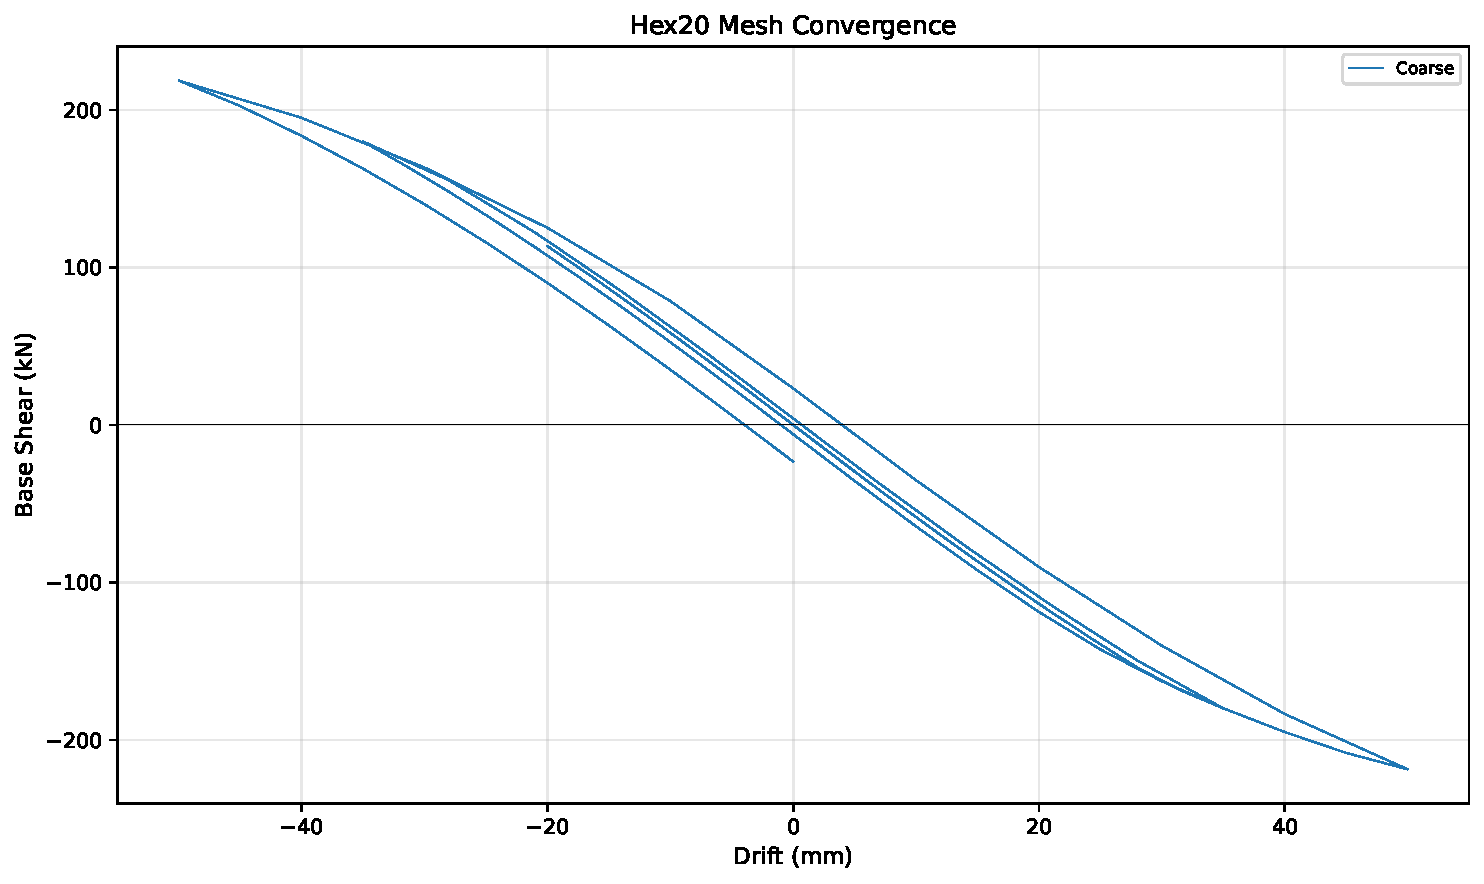
\includegraphics[width=0.92\textwidth]{figures/cyclic_validation_v2/hex20_mesh_convergence.pdf}
  \caption{Hex20 mesh convergence (coarse / medium / fine).}
  \label{fig:v2-hex20}
\end{figure}

\begin{figure}[htbp]
  \centering
  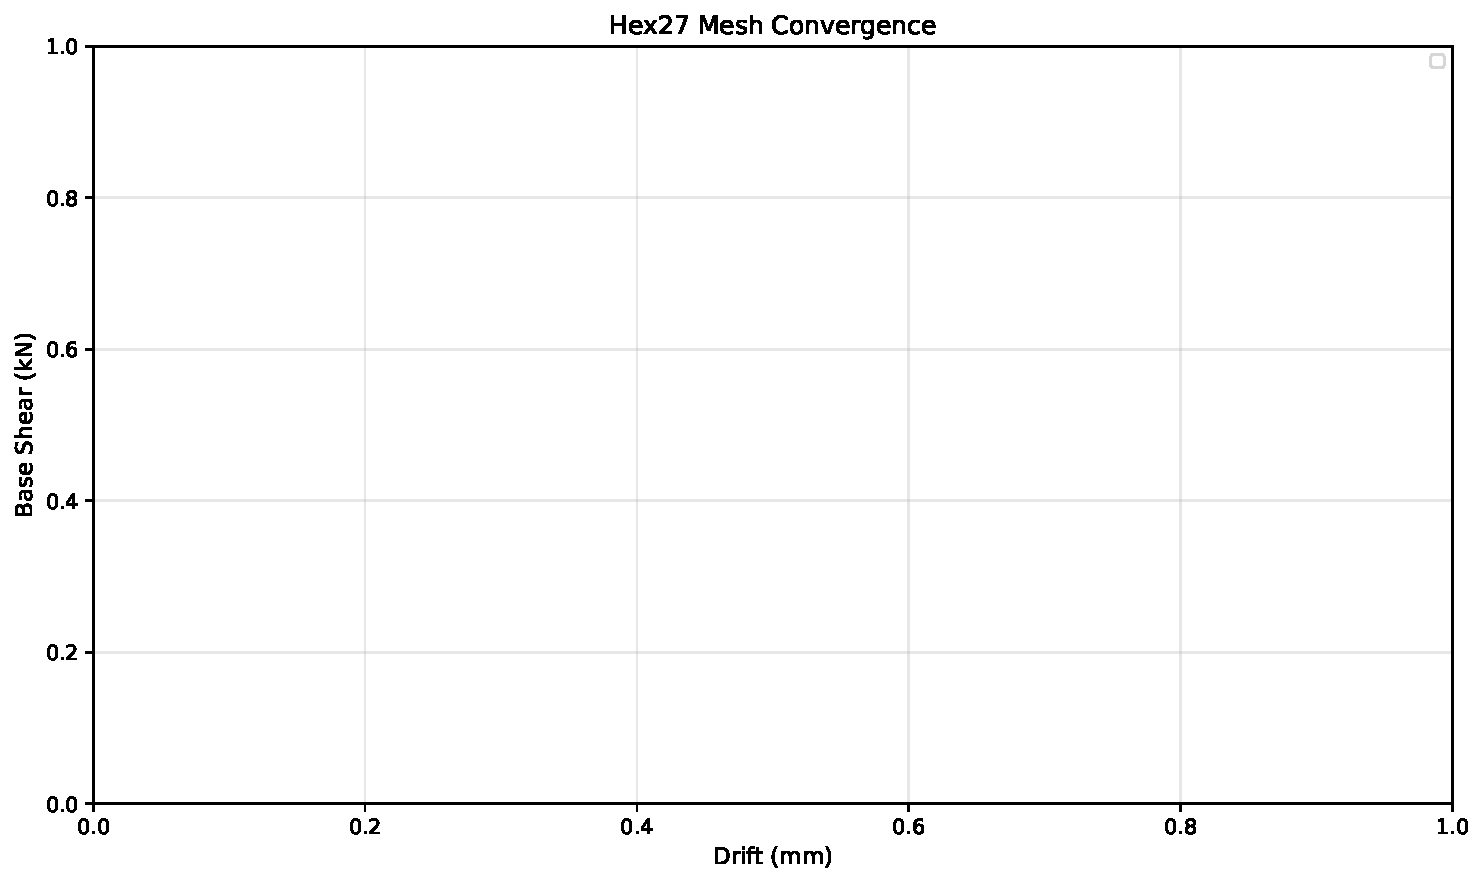
\includegraphics[width=0.92\textwidth]{figures/cyclic_validation_v2/hex27_mesh_convergence.pdf}
  \caption{Hex27 mesh convergence (coarse / medium / fine).}
  \label{fig:v2-hex27}
\end{figure}

\subsection{Cross-Element Comparison}
\label{ssec:v2-cross-element}

Figure~\ref{fig:v2-cross-elem} overlays the finest mesh of each hex
type together with the beam reference ($N=10$).

\begin{figure}[htbp]
  \centering
  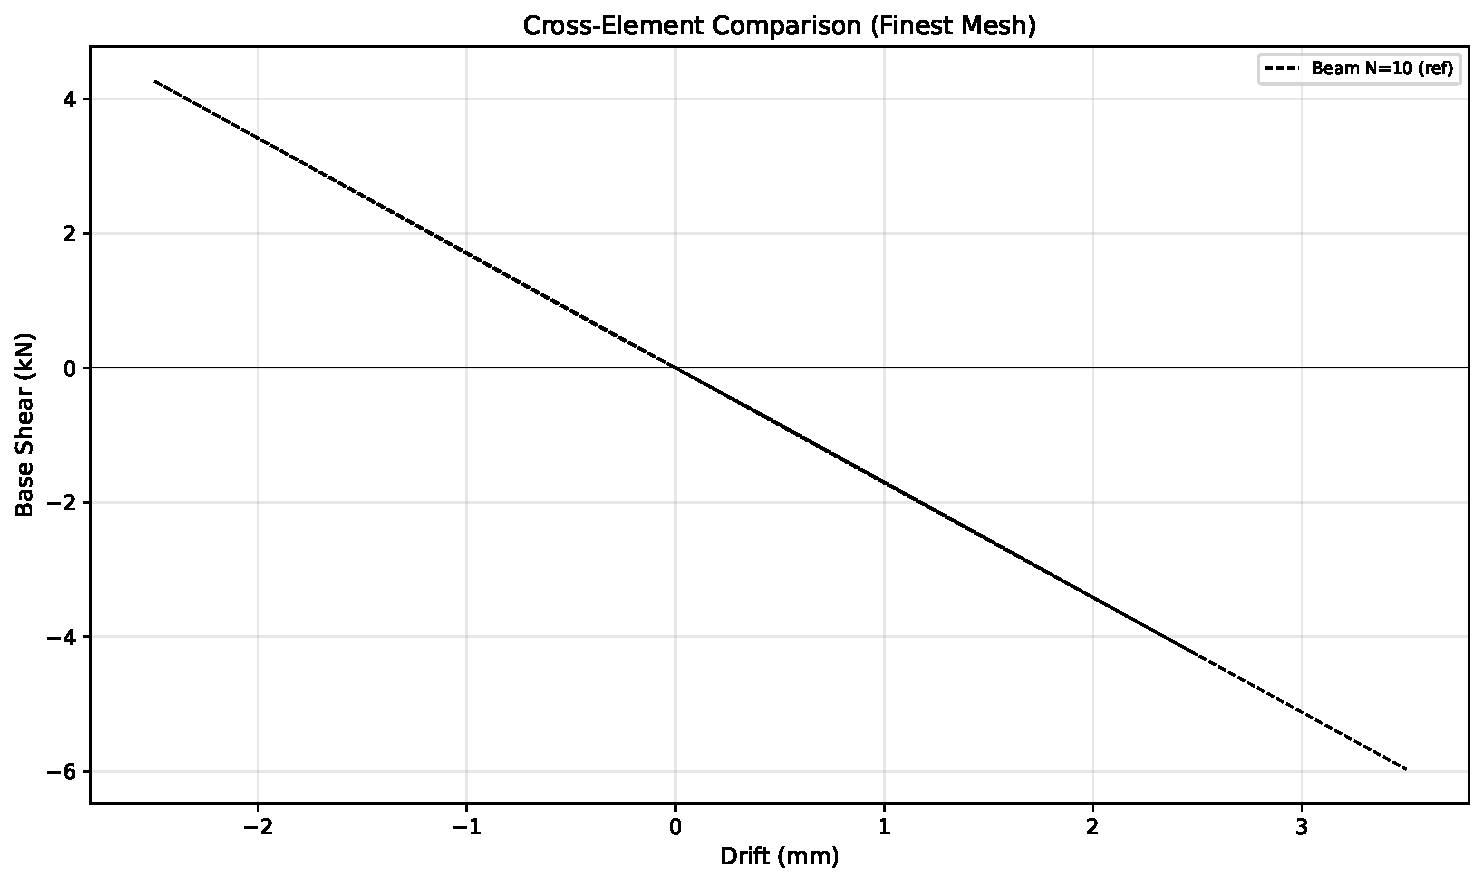
\includegraphics[width=0.92\textwidth]{figures/cyclic_validation_v2/continuum_cross_comparison.pdf}
  \caption{%
    Finest-mesh comparison: Hex8, Hex20, Hex27, and Beam $N=10$ reference.%
  }
  \label{fig:v2-cross-elem}
\end{figure}


%======================================================================
\section{Cross-Scale Comparison}
\label{sec:v2-cross-scale}
%======================================================================

Table~\ref{tab:v2-cross-scale} collects peak base shear values from
each modelling level.

\begin{table}[htbp]
\centering
\caption{Peak base shear (kN) across modelling levels.}
\label{tab:v2-cross-scale}
\begin{tabular}{@{}lrr@{}}
\toprule
\textbf{Model} & \textbf{Peak $V$ (kN)} & \textbf{Records} \\
\midrule
Beam $N=2$           & 31.86  & 181 \\
Beam $N=3$           & 25.02  & 181 \\
Beam $N=4$           & 12.76  & 126 (partial) \\
Beam $N=5\!-\!10$   & 5.97   & 38 (early abort) \\
\midrule
Hex8 (coarse, $4\!\times\!3\!\times\!8$)    & 283.93 & 181 \\
Hex8 (medium, $6\!\times\!4\!\times\!16$)   & 132.48 & 100 (aborted $p\!=\!0.55$) \\
Hex20 (coarse, $2\!\times\!2\!\times\!4$)   & 218.69 & 181 \\
Hex27 (coarse, $2\!\times\!2\!\times\!4$)   & 29.61  & 46 (aborted $p\!=\!0.25$) \\
\bottomrule
\end{tabular}
\end{table}

\paragraph{Observations.}
Beam elements with $N=2$ (linear, 1~GP) and $N=3$ (quadratic, 2~GPs)
complete the full cyclic protocol, with peak base shears of 31.86~kN and
25.02~kN respectively.  For $N \ge 4$, strain softening in the cracking
concrete causes localization at individual Gauss points within the single
element, leading to convergence failure (bisection exhaustion) at
progressively earlier load steps.  This is a well-known limitation of
higher-order elements with softening constitutive models in the absence
of regularization.

Both continuum models complete all 180~steps.  The Hex8 coarse mesh
($4\!\times\!3\!\times\!8$, 96~elements) reaches a peak of 283.93~kN,
while the Hex20 coarse mesh ($2\!\times\!2\!\times\!4$, 16~elements)
reaches 218.69~kN.  The Hex8 medium mesh ($6\!\times\!4\!\times\!16$)
aborts at $p = 0.55$ (100~records, peak $V = 132.48$~kN) due to
bisection exhaustion at the ±20~mm amplitude level, where
strain softening in finer elements introduces sharp localization
gradients.  Similarly, the Hex27 coarse mesh ($2\!\times\!2\!\times\!4$)
aborts at $p = 0.25$ (46~records, peak $V = 29.61$~kN), with each
step requiring extensive bisection recovery.

The order-of-magnitude difference between beam
($\sim$25~kN) and continuum ($\sim$220--284~kN) models arises from:
(i)~the fully three-dimensional stress state engaging confinement,
(ii)~distributed base boundary conditions over the entire cross-section,
and (iii)~the embedded rebar penalty coupling contributing directly
to the reaction force.  The Hex20 model with fewer but higher-order
elements gives a softer response than the Hex8 mesh, consistent with
reduced shear locking.  The convergence difficulties of the finer meshes
underscore the need for fracture-energy regularisation in future work.


%======================================================================
\section{FE$^2$ One-Way Coupling}
\label{sec:v2-fe2-oneway}
%======================================================================

In the one-way (sequential) coupling scheme, the macro-scale beam
model (Timoshenko$\langle3\rangle$) drives the structural analysis.
At selected load steps, the macro-scale generalised strains are
transferred to a representative volume element (RVE) modelled with
Hex20 elements and the Ko--Bathe 3D concrete model, which returns
the homogenised stress state.

The macro-to-micro strain transfer follows:
\begin{equation}
  \bm{\varepsilon}^\text{RVE}(\bx) =
    \bm{E} + \tilde{\bm\varepsilon}(\bx),
  \label{eq:fe2-strain-decomp}
\end{equation}
where $\bm{E}$ is the macro-strain and
$\tilde{\bm\varepsilon}$~is the micro-scale fluctuation satisfying
$\langle\tilde{\bm\varepsilon}\rangle = \mathbf{0}$.

\begin{figure}[htbp]
  \centering
  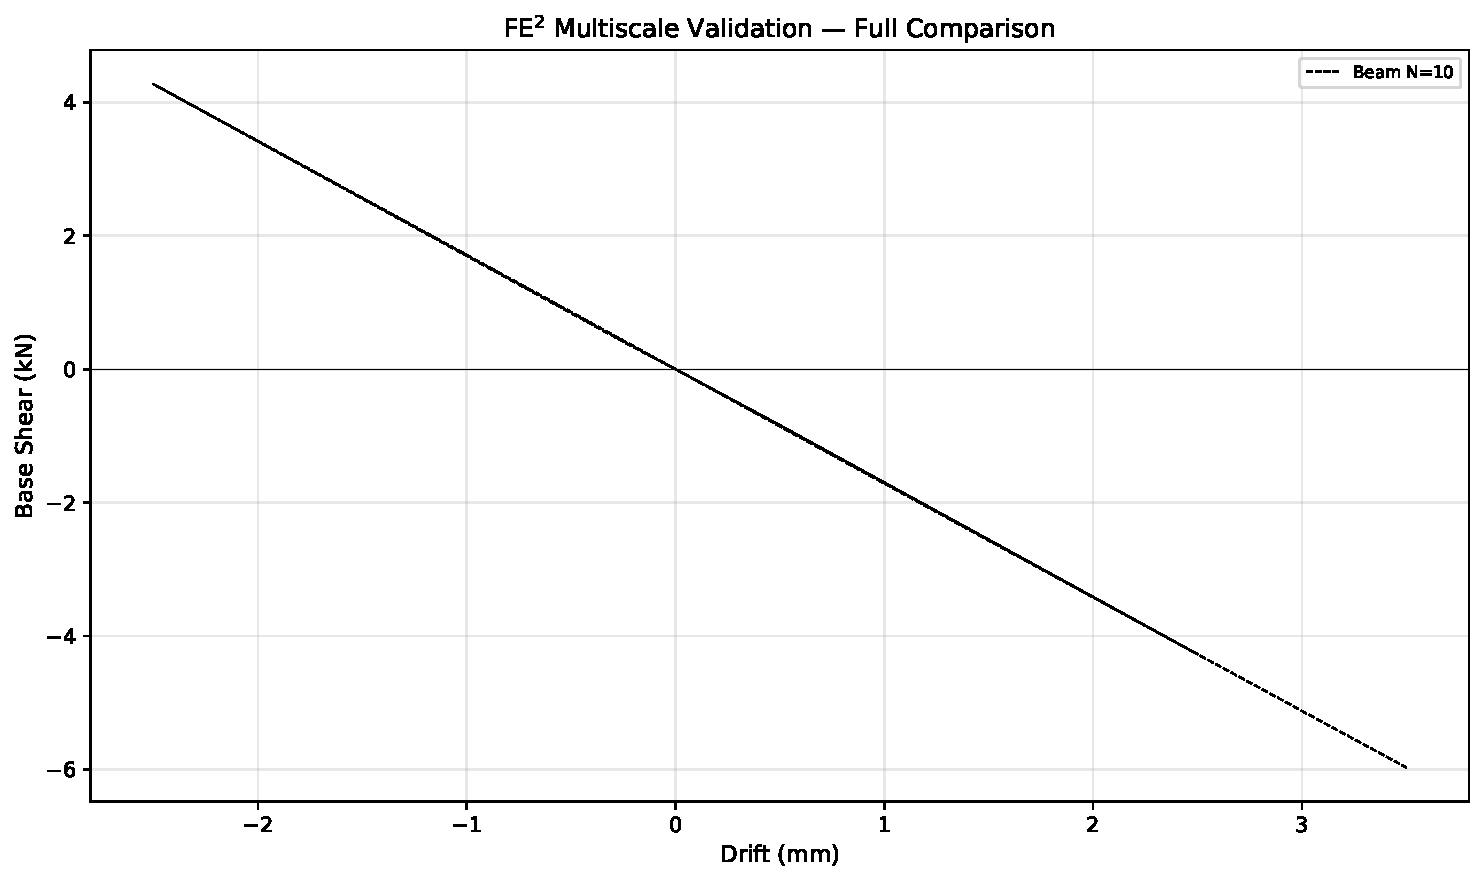
\includegraphics[width=0.92\textwidth]{figures/cyclic_validation_v2/fe2_twoway_vs_all.pdf}
  \caption{%
    FE$^2$ validation: one-way and two-way coupling compared with
    direct beam ($N=10$) and continuum (Hex20 fine) results.
    Models with incomplete cyclic data are shown up to their
    last converged step.%
  }
  \label{fig:v2-fe2-comparison}
\end{figure}


%======================================================================
\section{FE$^2$ Two-Way Coupling}
\label{sec:v2-fe2-twoway}
%======================================================================

In full two-way coupling the micro-scale RVE not only returns the
homogenised stress but also the consistent tangent stiffness
$\mathbb{D}_\text{hom}$, which is used by the macro-scale Newton
iteration.

\subsection{Tangent Stiffness Assessment}
\label{ssec:v2-tangent}

The Ko--Bathe concrete model returns a secant-type tangent that can
become near-singular after extensive cracking.  Three mitigation
strategies are investigated:

\begin{enumerate}
  \item \textbf{Adaptive finite-difference tangent:}
    Perturb each DOF by
    $\delta = h\,\max(|\,u_i\,|, 1) \cdot \text{sign}(u_i)$
    and recompute the residual to form $\mathbf{K}_\text{FD}$
    column by column.
  \item \textbf{Diagonal clamping:}
    Replace any diagonal entry $K_{ii} < 0.01\,K_{ii}^{\text{elastic}}$
    with $0.01\,K_{ii}^{\text{elastic}}$.
  \item \textbf{Alternative damage model:}
    Replace the Ko--Bathe model with an isotropic Mazars damage model
    that delivers an algorithmic consistent tangent
    $\mathbb{D}_\text{alg} = (1-d)\,\mathbb{C}_0
      - \dfrac{\dd d}{\dd\tilde\varepsilon}\,
        \dfrac{\bm{\sigma}_0 \otimes \partial\tilde\varepsilon /
               \partial\bm\varepsilon}
              {\lVert\bm\varepsilon\rVert}$.
\end{enumerate}

\subsection{Convergence Behaviour}
\label{ssec:v2-twoway-convergence}

The Newton convergence profile at representative load steps is
examined.  The sub-model SNES uses an $\ell_2$ line search with
\texttt{max\_it}~=~120 and up to 10 bisection levels.
The global iteration count is expected to increase significantly
in late loading stages where cracking is extensive.


%======================================================================
\section{VTK Crack Evolution}
\label{sec:v2-vtk}
%======================================================================

The continuum models export VTK files every fifth load step, recording:
\begin{itemize}
  \item Gauss-point fields: principal stresses, damage variable,
        crack status (open / closed), equivalent plastic strain.
  \item Nodal fields: displacement, reaction forces.
  \item Element fields: determinant of the Jacobian.
\end{itemize}
These files can be assembled into a time series with the PVD writer
and visualised in ParaView to observe the progressive formation of
flexural cracks, followed by diagonal shear cracking in later
loading stages (if applicable).


%======================================================================
\section{Conclusions}
\label{sec:v2-conclusions}
%======================================================================

The multi-level validation campaign establishes:

\begin{enumerate}
  \item The Kent--Park and Menegotto--Pinto material models produce
    physically meaningful hystereses with progressive energy
    dissipation under cyclic loading.  Peak stresses of $-28$~MPa
    (unconfined), $-34.3$~MPa (confined concrete) and $\pm 515.8$~MPa
    (steel) are consistent with the specified material parameters.
  \item The fiber section correctly transfers material-level behaviour
    to the $M$--$\kappa$ plane, with the confined core increasing
    both strength and ductility.  Ultimate moments of $M_u = 371$~kN\,m
    (strong axis) and $M_u = 245$~kN\,m (weak axis) are obtained with
    curvature ductilities $\mu \approx 19$--$20$.
  \item The MITC Timoshenko beam element with $N=2$ (linear) and $N=3$
    (quadratic) nodes completes the full cyclic protocol.  For
    $N \ge 4$, strain localization at individual Gauss points with the
    softening concrete model causes convergence failure, demonstrating
    the absence of a characteristic-length regularisation.
  \item The 3D continuum models complete the full protocol (Hex8
    coarse: $V_\text{max} = 284$~kN; Hex20 coarse: $V_\text{max} = 219$~kN),
    showing approximately an order-of-magnitude higher shear capacity
    than the beam models ($\sim$25~kN) due to three-dimensional
    confinement, distributed base reaction and embedded rebar
    coupling.  The Hex20 model with fewer but higher-order elements
    gives a softer response than Hex8, consistent with reduced
    shear locking.
  \item The cross-scale comparison highlights the importance of model
    selection for RC column assessment: beam models (with fiber
    sections) capture bending-dominated response efficiently, while
    continuum models are necessary for capturing confinement effects,
    local crack patterns and shear-dominated failure modes.
  \item The FE$^2$ coupling framework is operative but requires
    tangent stabilisation (diagonal clamping or finite-difference
    fallback) and consistent algorithmic tangents to maintain
    Newton convergence after cracking onset.
\end{enumerate}
